\begin{center}
\begin{minipage}{\linewidth}\centering
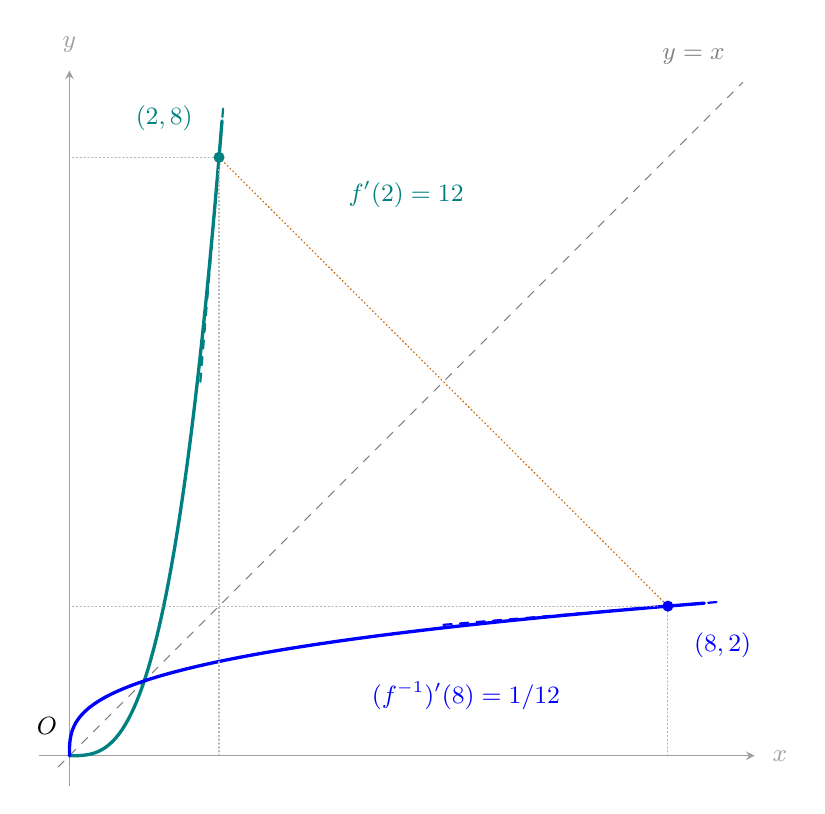
\begin{tikzpicture}[x=0.95cm,y=0.95cm,>=stealth,font=\small,line cap=round,line join=round]
\draw[->,gray!75] (-0.4,0)--(9.16,0) node[right=3pt]{$x$};
\draw[->,gray!75] (0,-0.4)--(0,9.16) node[above=3pt]{$y$};
\node at (-.3,.4) {$O$};
\draw[gray,dashed] (-0.15,-0.15)--(9,9) node[above left=3pt]{$y=x$};

\draw[teal,very thick,domain=0:2.04,samples=121] plot(\x,{\x^3});
\draw[blue,very thick,domain=0:2.04,samples=121] plot({\x^3},\x);
\draw[gray!60,densely dotted] (2,0)--(2,8)--(0,8) (8,0)--(8,2)--(0,2);
\draw[orange!80!black,densely dotted] (2,8)--(8,2);
\draw[teal,dashed,thick] (1.75,5)--(2.06,8.72);
\draw[blue,dashed,thick] (5,1.75)--(8.72,2.06);
\fill[teal] (2,8) circle(2pt) node[above left=6pt]{$(2,8)$};
\fill[blue] (8,2) circle(2pt) node[below right=6pt]{$(8,2)$};
\node[teal] at (4.5,7.5) {$f'(2)=12$};
\node[blue] at (5.3,.8) {$(f^{-1})'(8)=1/12$};

\end{tikzpicture}\par\smallskip
{\small \textcolor{teal}{\rule[.5ex]{1em}{.8pt}\ $y=x^3$}\qquad\textcolor{blue}{\rule[.5ex]{1em}{.8pt}\ $y=\sqrt[3]{x}$}}\par
{\small 先配对原函数上的点 $(2,8)$ 与镜像点 $(8,2)$，再取切线斜率的倒数。}\par\smallskip
\end{minipage}
\end{center}
